\chapter{Gestion de projet}\label{ch:gestion-projet}

Pendant mon alternance, j'ai très vite compris que pour l'entreprise, il est important de maintenir son esprit innovant, de constamment générer davantage de valeur, et d'être à l'écoute tout en s'ajustant selon les exigences de sa clientèle. La politique d'innovation de l'entreprise repose sur les recommandations émanant à la fois de ses clients et de ses collaborateurs. Un comité dédié à l'innovation se rassemble hebdomadairement pour examiner les suggestions les plus récentes. Chaque concept est traité, trié et priorisé. Il s'agit d'un processus en plusieurs étapes qui implique également d'autres comités, comme l'illustre la Figure~\ref{fig:committees} et la Table~\ref{tblr:character-committees}. Par la suite, l'ensemble de ces propositions est transmis au département Recherche et Développement en vue de la création de nouvelles fonctionnalités. Tous les quatre mois, de nouvelles options viennent enrichir l'ensemble des services, désignées sous le terme ``Editions''.

\begin{figure}[h]
    \centering
    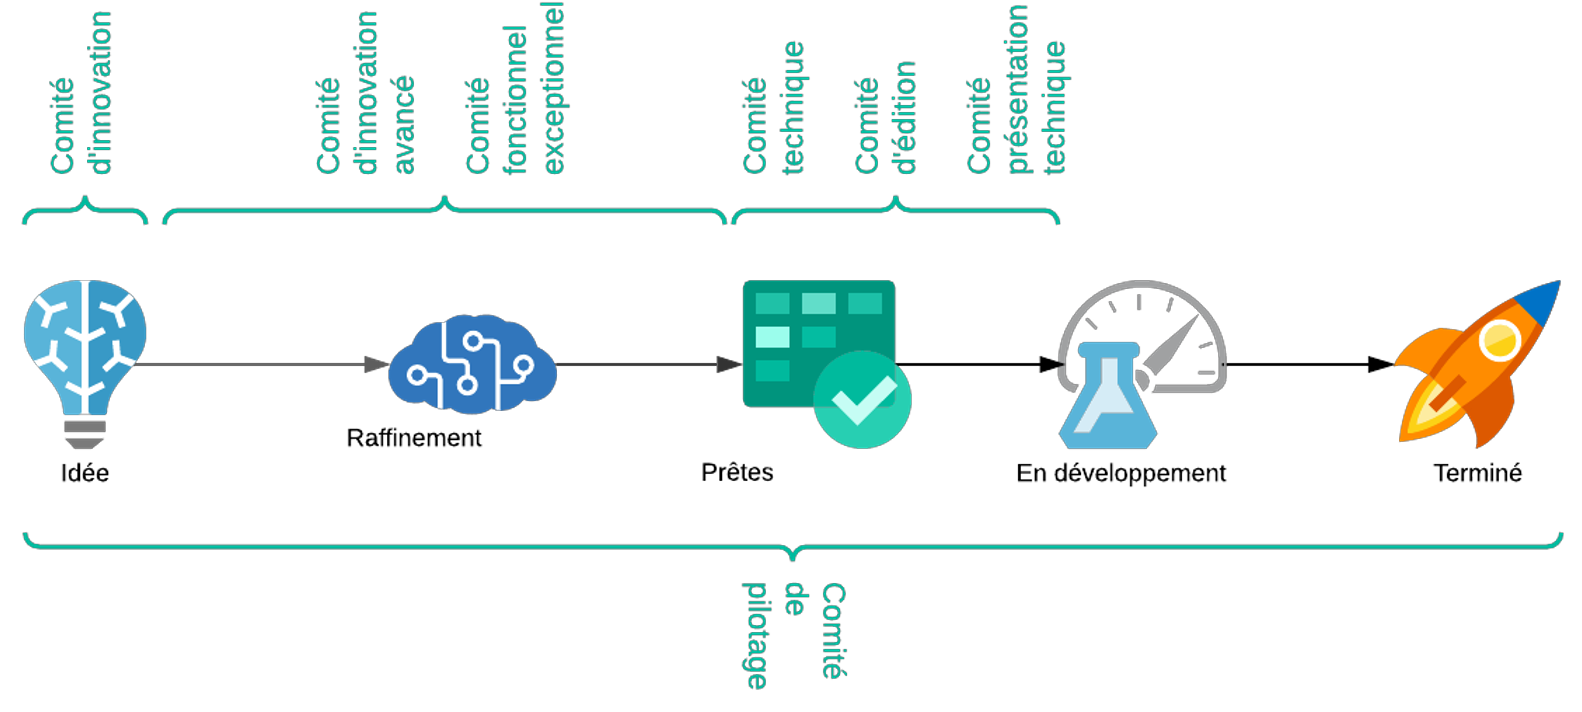
\includegraphics[width=\textwidth]{img/committees}
    \caption{La participation des différents comités au processus de traitement des idées d'innovation.}
    \label{fig:committees}
\end{figure}

Une édition représente le fruit de quatre mois de travail de développement, cependant, son élaboration ne s'arrête pas là. Elle englobe la mise en place et la planification des activités de communication (marketing), la formation des équipes support et commerce, la rédaction de manuels et de tutoriels destinés aux clients, ainsi que la préparation des prochaines éditions à venir.

\begin{longtblr}[
    caption={Les caractéristiques des différents comités.},
    label={tblr:character-committees}
    ]{
    hlines,vlines,
    rowspec={Q[m,font=\footnotesize\bfseries,gray9]*{7}{Q[m,font=\footnotesize]}}
    }
    {Nom du        \\ comité}       & {Récur-\\rence}   & Objectif          & Entrées & Sorties \\
    {Comité        \\ d'innovation} & {Hebdo-\\madaire} & {Première analyse                     \\ des idées exprimées                     \\ puis étude de l'intérêt \\ de chaque idée.} & {Liste des \\ idées} & {Idées clarifiées, \\ note par niveau \\ d'intérêt} \\
    {Comité        \\ d'innovation \\ avancé} & Mensuel & {Clarifier les \\ spécifications \\ fonctionnelles des \\ idées exprimées au \\ cours des comités \\ d'innovations.} & {Ordre du jour \\ des idées, déjà \\ analysées} & {Réponses aux \\ questions \\ à l'ordre du \\ jour, ajoutées \\ aux backlog} \\
    {Comité        \\ fonctionnel \\ exceptionnel} & {Excep-\\tionnel} & {Le PO sollicite une \\ partie prenante \\ identifiée, qui devrait \\ lui permettre de \\ lever un certain \\ nombre de questions \\ autour d'une \\ fonctionnalité.} & {Fonctionnalités, \\ déjà analysées \\ et comportant \\ toujours \\ des questions} & {Les réponses \\ sont ajoutées \\ aux \\ fonctionnalités} \\
    {Comité        \\ tech} & {En fonction \\ des items \\ en attente \\ de chiffrage \\ dans le \\ backlog. \\ Au moins \\ hebdo-\\madaire.} & {Une présentation \\ des items, validés \\ fonctionnellement, \\ pour faire ressortir \\ un macro-chiffrage, \\ réalisé par l'équipe \\ d'expert.} & {Fonctionnalités \\ prêtes du \\ backlog \\ produit} & {Macro-chiffrage \\ ou questions \\ fonctionnelles} \\
    {Comité        \\ pilotage} & {Bimestriel} & {Donner une vision \\ claire de l'avancement \\ du travail réalisé \\ pour les services \\ concernés.} & {Indicateur clé \\ de performance \\ à partager} & {Adaptations \\ à mettre en \\ œuvre} \\
    {Comité        \\ d'édition} & {Bimestriel} & {Établir une \\ constitution \\ d'édition à partir \\ des idées prêtes. \\ En déduire un \\ objectif d'édition \\ permettant de \\ fédérer autour \\ d'une réalisation.} & {Fonctionnalités \\ prêtes, analyse du \\ temps disponible \\ faite à partir \\ des paramètres \\ vélocité / nombre \\ de demandes \\ courantes / dette \\ technique \dots
    } & {Liste des \\ composants \\ d'édition, \\ objectif \\ d'édition} \\
    {Comité        \\ présentation \\ technique /\\ Kickoff \\ Edition} & {En début \\ d'édition} & {Une présentation des \\ items embarqués dans \\ l'édition, ainsi qu'un \\ focus sur l'objectif \\ d'édition.} & {L'objectif, \\ le contenu \\ d'édition} & {Le retour \\ de l'équipe \\ sur le contenu \\ et l'objectif}
\end{longtblr}

\section{Méthodologie Agile}\label{sec:agile}

L'équipe de développement de la géolocalisation de SuiviDeFlotte -- comme les autres équipes de développement de l'entreprise -- travaille selon la méthodologie agile SCRUM. Cette méthodologie est une approche de gestion de projet qui met l'accent sur la flexibilité, la collaboration et la livraison continue. Elle est largement utilisée dans le développement de logiciels et peut également être appliquée à d'autres domaines. SCRUM divise un projet en cycles appelés \foreignquote{french}{itérations} ou \foreignquote{french}{sprints} de courte durée, généralement de deux à quatre semaines, pendant lesquels une partie du travail est accomplie et livrée.

Les termes clés de la méthodologie SCRUM sont énumérés ci-dessous et illustrés dans la Figure~\ref{fig:agile}.

\begin{description}
    \item[Product Owner (Propriétaire du Produit)] La personne responsable de définir et de prioriser les éléments du produit à développer. Le Propriétaire du Produit représente les besoins des utilisateurs et des parties prenantes.
    \item[Scrum Master (Maître de Scrum)] Le facilitateur du processus SCRUM. Le Scrum Master s'assure que l'équipe suit les principes SCRUM, élimine les obstacles et favorise un environnement de travail efficace.
    \item[Équipe de Développement] Le groupe de professionnels chargé de concevoir, développer, tester et livrer les éléments du produit à la fin de chaque sprint.
    \item[User Story (Histoire Utilisateur)] Une Histoire Utilisateur est une courte description d'une fonctionnalité ou d'un aspect du produit, racontée du point de vue de l'utilisateur. Elle suit généralement le format \foreignquote{french}{En tant que [utilisateur], je veux [action] afin de [objectif]}. Les Histoires Utilisateurs sont des éléments du Carnet de Produit et aident à définir les fonctionnalités du produit du point de vue de l'utilisateur.
    \item[Story Point (Point d'Histoire)] Le Point d'Histoire est une unité relative utilisée pour estimer la complexité, l'effort et la taille des Histoires Utilisateurs ou des tâches de développement. Il n'a pas de valeur absolue, mais il sert à comparer la difficulté relative entre différentes Histoires Utilisateurs. Les équipes de développement attribuent des points d'histoire lors des estimations, ce qui les aide à planifier la quantité de travail qu'elles peuvent accomplir dans un sprint donné.
    \item[Epic (Épique)] Un Épic est une unité de travail plus large que les Histoires Utilisateurs individuelles. Il représente généralement un ensemble de fonctionnalités, de tâches ou de travaux qui sont trop importants pour être traités dans un seul sprint. Les Épics sont souvent des objectifs à long terme qui sont décomposés en Histoires Utilisateurs plus petites et gérables. Ils aident à organiser et à structurer le développement du produit en regroupant des éléments liés autour d'un thème ou d'un objectif commun. Les Épics sont inclus dans le Carnet de Produit et sont priorisés en fonction de leur valeur pour l'utilisateur et du contexte global du projet.
\end{description}

SCRUM encourage la transparence, l'adaptabilité et la collaboration continue entre les membres de l'équipe et les parties prenantes, ce qui permet de s'adapter aux changements et de fournir rapidement de la valeur tout au long du projet.

\begin{figure}[ht]
    \centering
    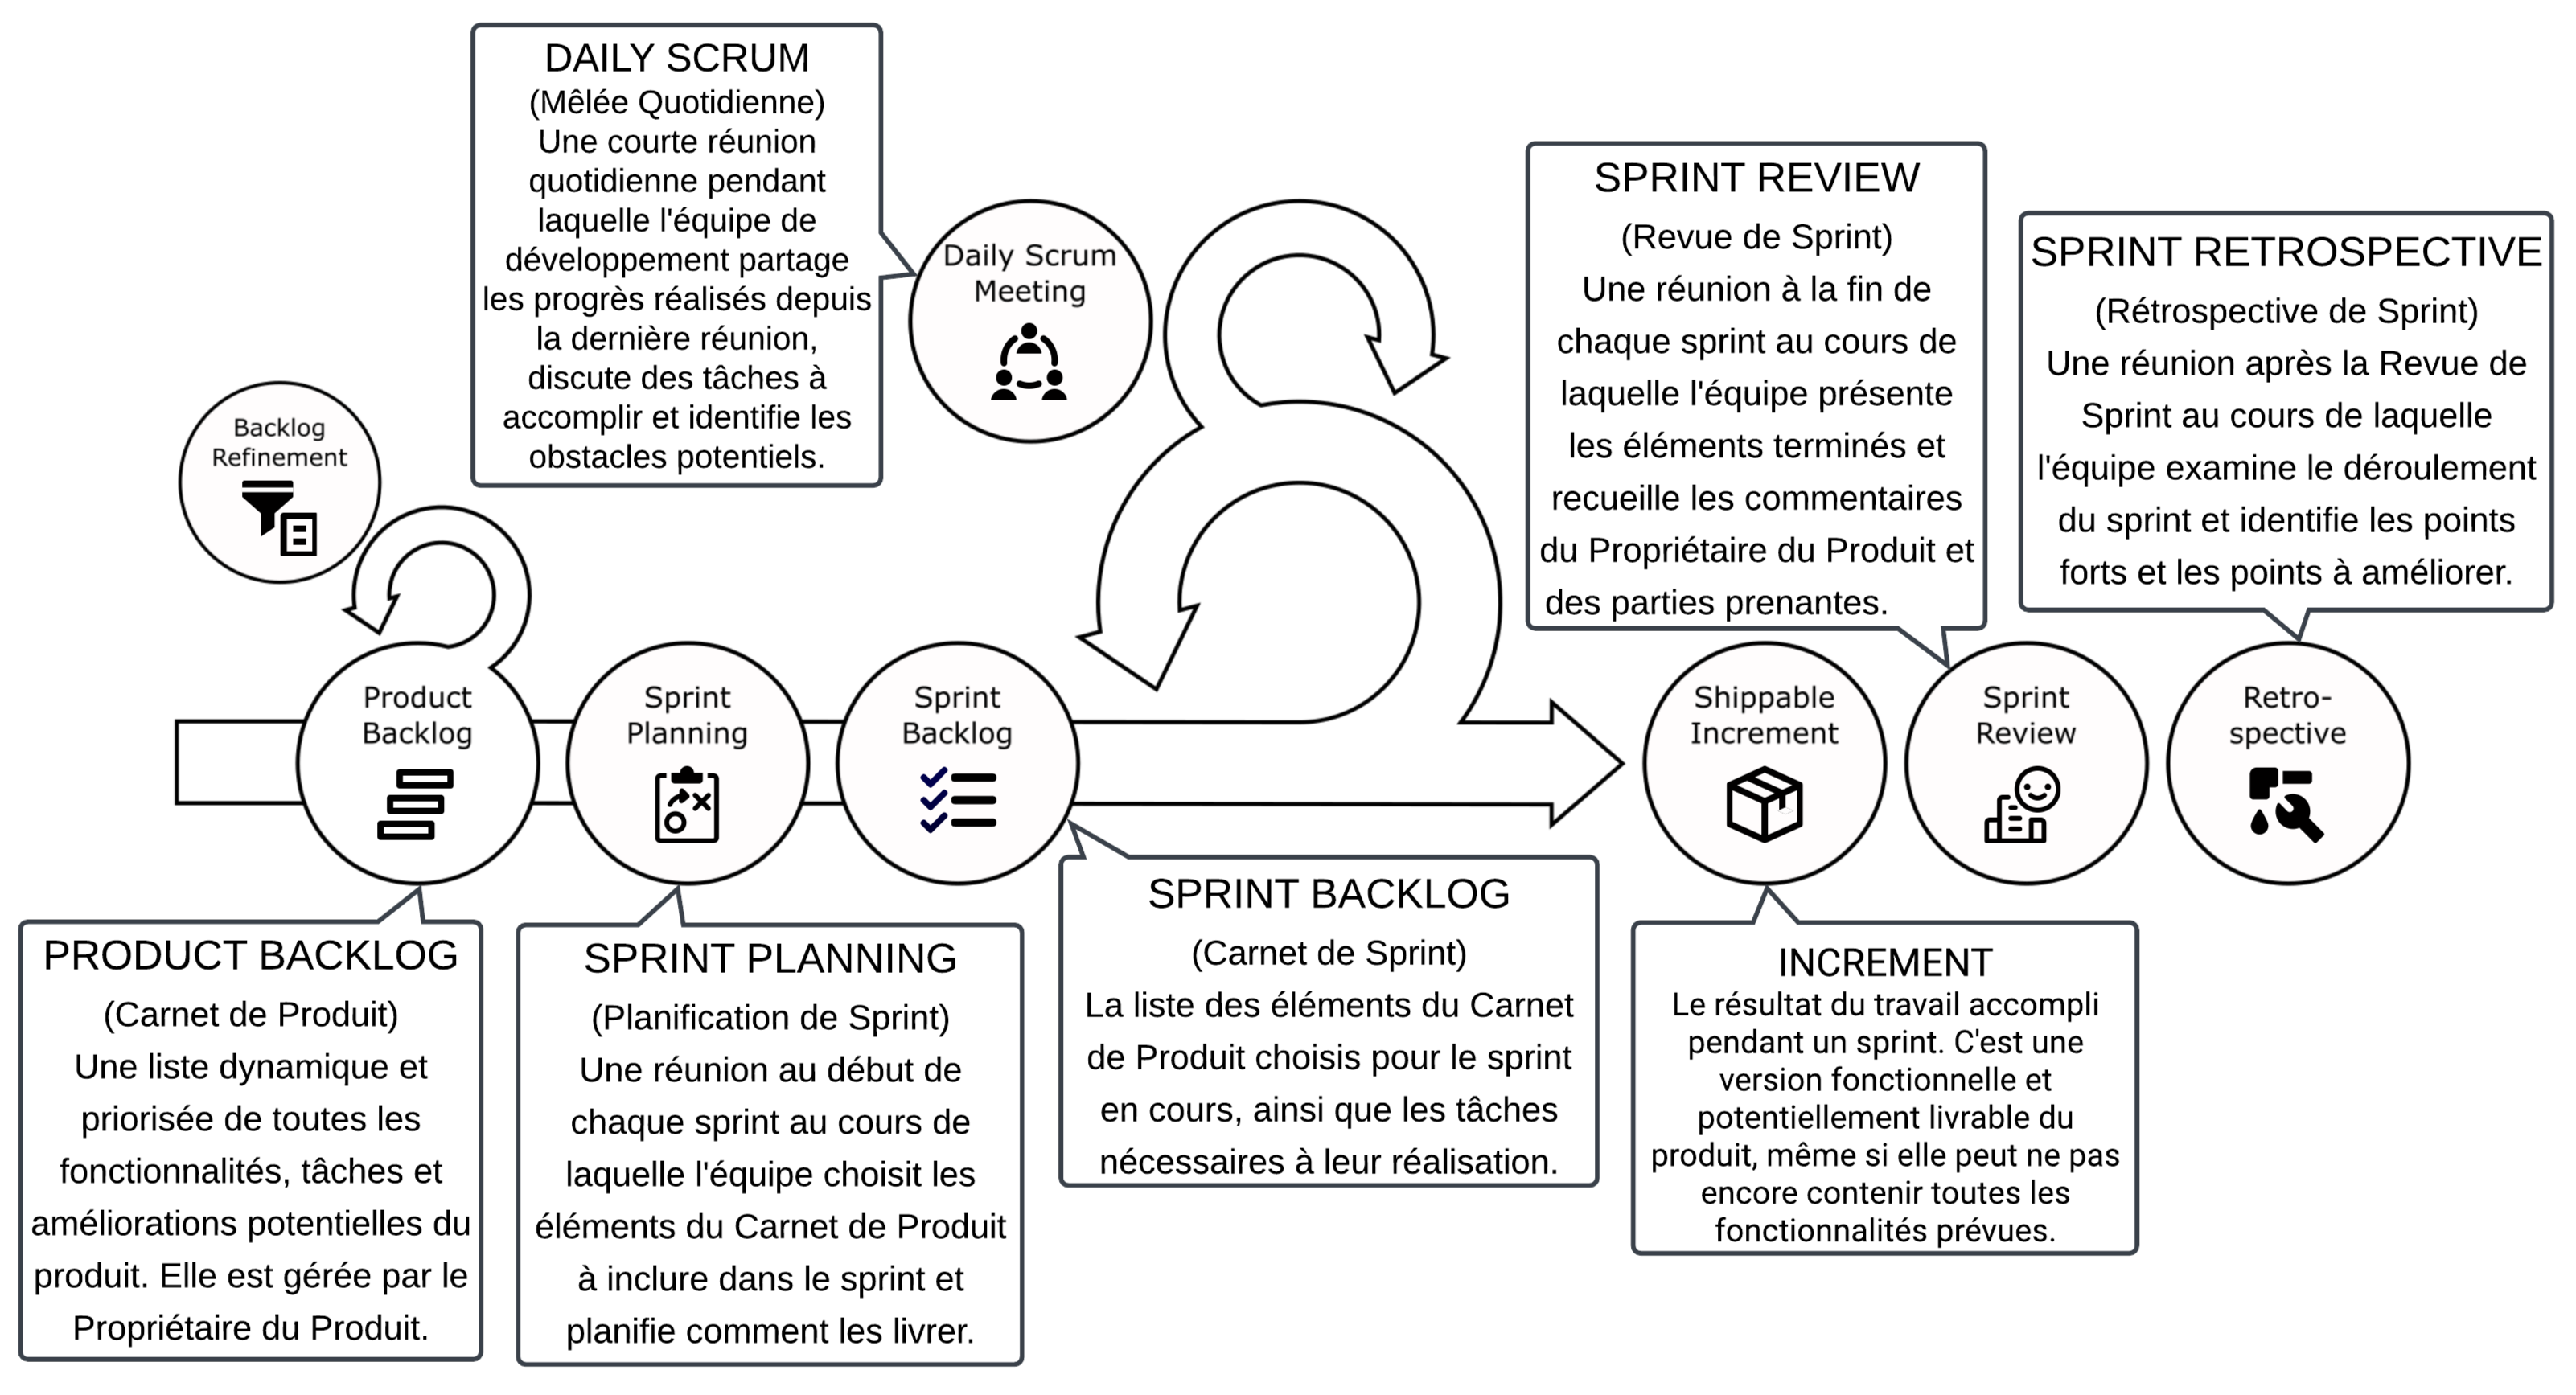
\includegraphics[width=\textwidth]{img/agile-02}
    \caption{Cérémonies SCRUM.}
    \label{fig:agile}
\end{figure}

Dans l'équipe Géoloc, le processus suit un calendrier de sprints de deux semaines (Figure~\ref{fig:sprint}). Chaque cycle commence par un ensemble de réunions clés qui ont lieu tous les deuxièmes mardis. Cette journée englobe la Revue de Sprint, la Rétrospective de Sprint et la Planification de Sprint. Lors de la Revue de Sprint, les éléments achevés sont présentés au Propriétaire du Produit et aux parties prenantes, les retours sont recueillis et les priorités sont ajustées si nécessaire. La Rétrospective de Sprint offre l'opportunité à l'équipe de réfléchir aux succès et d'identifier les domaines à améliorer, favorisant une culture d'amélioration continue. Ensuite, la Planification de Sprint implique la sélection des Histoires Utilisateurs du Carnet de Produit à inclure dans le sprint à venir, en tenant compte de leur complexité et de leur priorité. Pour l'estimation de la complexité des tâches, des Points d'Histoire basés sur la séquence de Fibonacci (1, 2, 3, 5, 8, 13) sont utilisés. Cette approche aide à attribuer des valeurs relatives à différentes tâches et assure une évaluation cohérente de la charge de travail.

À la fin de chaque sprint, les nouveaux incréments sont également mis en production. Grâce à l'approche Agile et à la fréquence des mises en production, les modifications apportées à l'application sont rapidement portées à la connaissance de l'utilisateur.

Chaque jour ouvrable débute par une Mêlée Quotidienne de 15 minutes, au cours de laquelle les progrès depuis la dernière réunion sont passés en revue, les tâches sont discutées et les obstacles potentiels sont identifiés. Ces réunions se déroulent généralement en ligne via Google Meet pour accueillir les collègues travaillant à distance et garantir la participation de tous les membres de l'équipe, peu importe leur emplacement. Par contre, pour maintenir la communication et la cohésion de l'équipe, les réunions du mardi de chaque deuxième semaine sont des réunions en personne. Cette pratique encourage les échanges directs, la collaboration étroite entre les membres de l'équipe et facilite la résolution rapide de tout problème ou obstacle pouvant survenir.

\begin{figure}[ht]
    \centering
    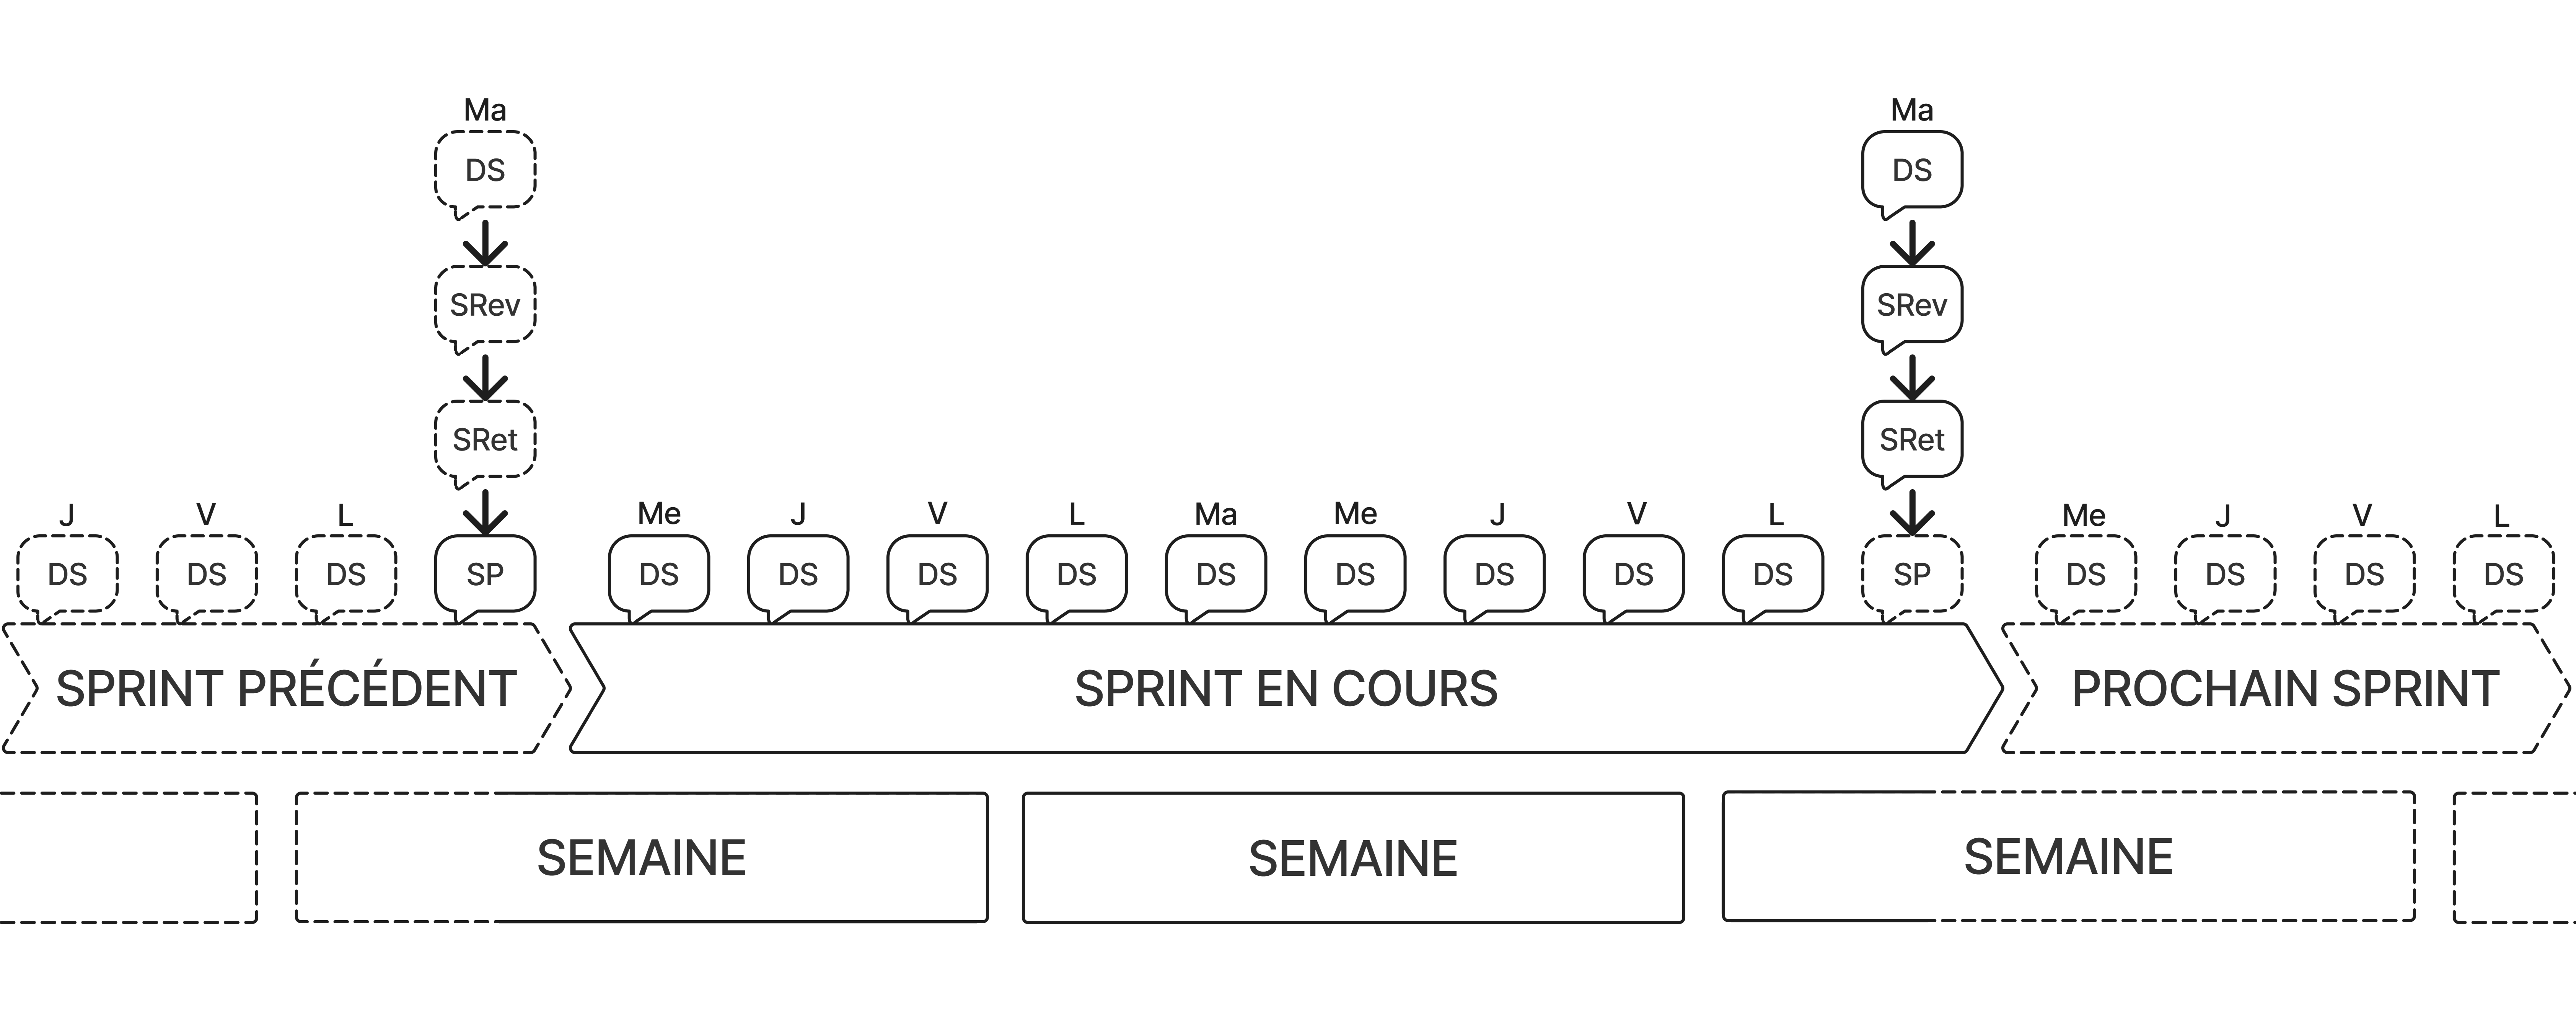
\includegraphics[width=\textwidth]{img/sprint04}
    \caption{Programme des sprints chez SuiviDeFlotte. Légende : L, Ma, Me, J, V -- jours de la semaine ; DS -- Daily Scrum ; SRev -- Sprint Review ; Sret -- Sprint Retrospective ; SP -- Sprint Planning ; ligne pointillée -- Sprint précédent ou suivant ; ligne continue -- Sprint en cours.}
    \label{fig:sprint}
\end{figure}

Actuellement, les rôles du Propriétaire du Produit et du Maître de Scrum ont été temporairement fusionnés en une seule personne. Cette configuration permet au Propriétaire du Produit de gérer les responsabilités du projet tout en facilitant le processus SCRUM, en maintenant une communication fluide avec l'équipe de développement.

En complément des cycles de deux semaines des Sprints, l'opération de l'entreprise comprend également un cycle plus long. En effet, comme je l'ai mentionné dans l'introduction de ce chapitre, l'entreprise publie une nouvelle version, appelée nouvelle Edition, de ses services en ligne tous les quatre mois, soit trois fois par an. Cela implique qu'il y a environ huit sprints pour que les développeurs puissent concevoir les nouvelles fonctionnalités des nouvelles éditions.

La Figure~\ref{fig:committees-and-scrum} résume les relations entre les comités et le processus des sprints. Comme on peut le voir, les tickets du Carnet de produit proviennent du Comité d'innovation, du Comité d'innovation avancée, du Comité fonctionnel exceptionnel, du Comité d'édition et du Comité d'innovation technique. Ensuite, le Comité d'édition sélectionne les tickets pour la prochaine Edition et le Comité de présentation technique les présente à l'équipe de développeurs. Une autre source de tickets dans le Backlog de Produit est l'équipe de support qui crée des tickets de bogues. Le traitement des bogues est illustré par la Figure~\ref{fig:treatment-of-bugs}. La section suivante explique comment ces tickets sont traités dans un outil appelé Jira.

\begin{figure}[ht]
    \centering
    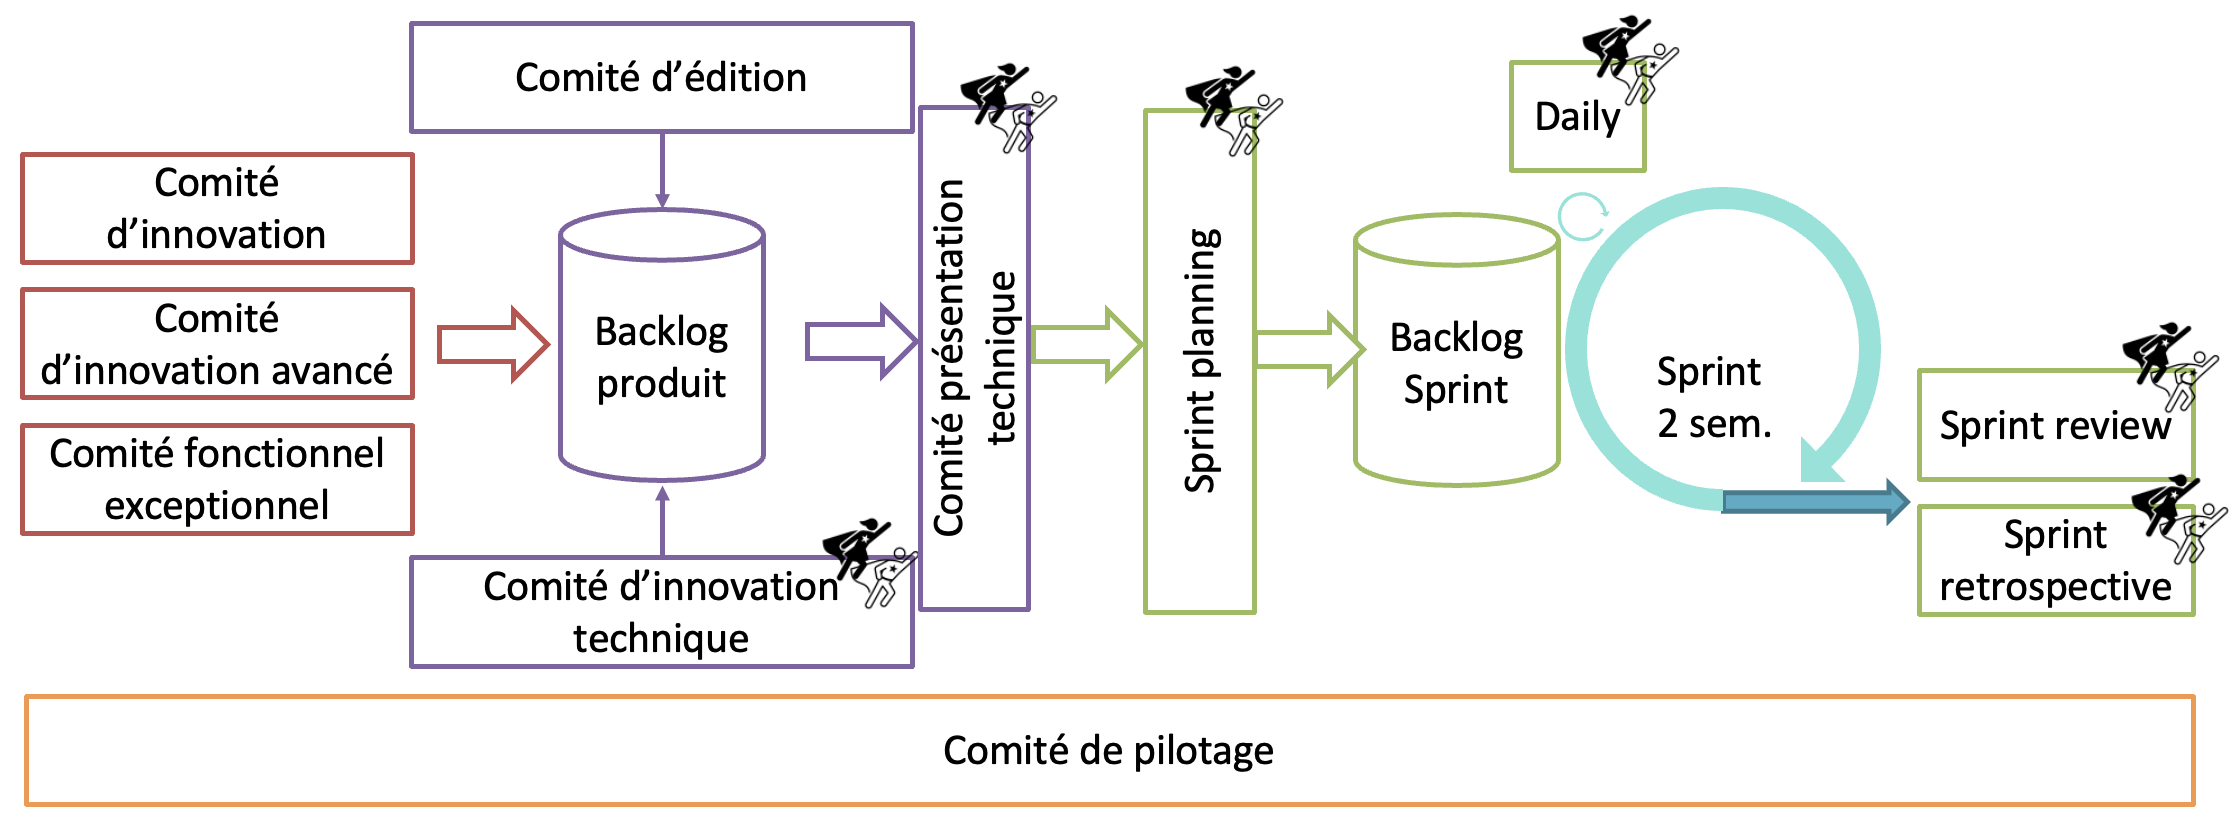
\includegraphics[width=\textwidth]{img/committees-and-scrum}
    \caption{Résumé des relations entre les comités et le processus des sprints.}
    \label{fig:committees-and-scrum}
\end{figure}

\begin{figure}[ht]
    \centering
    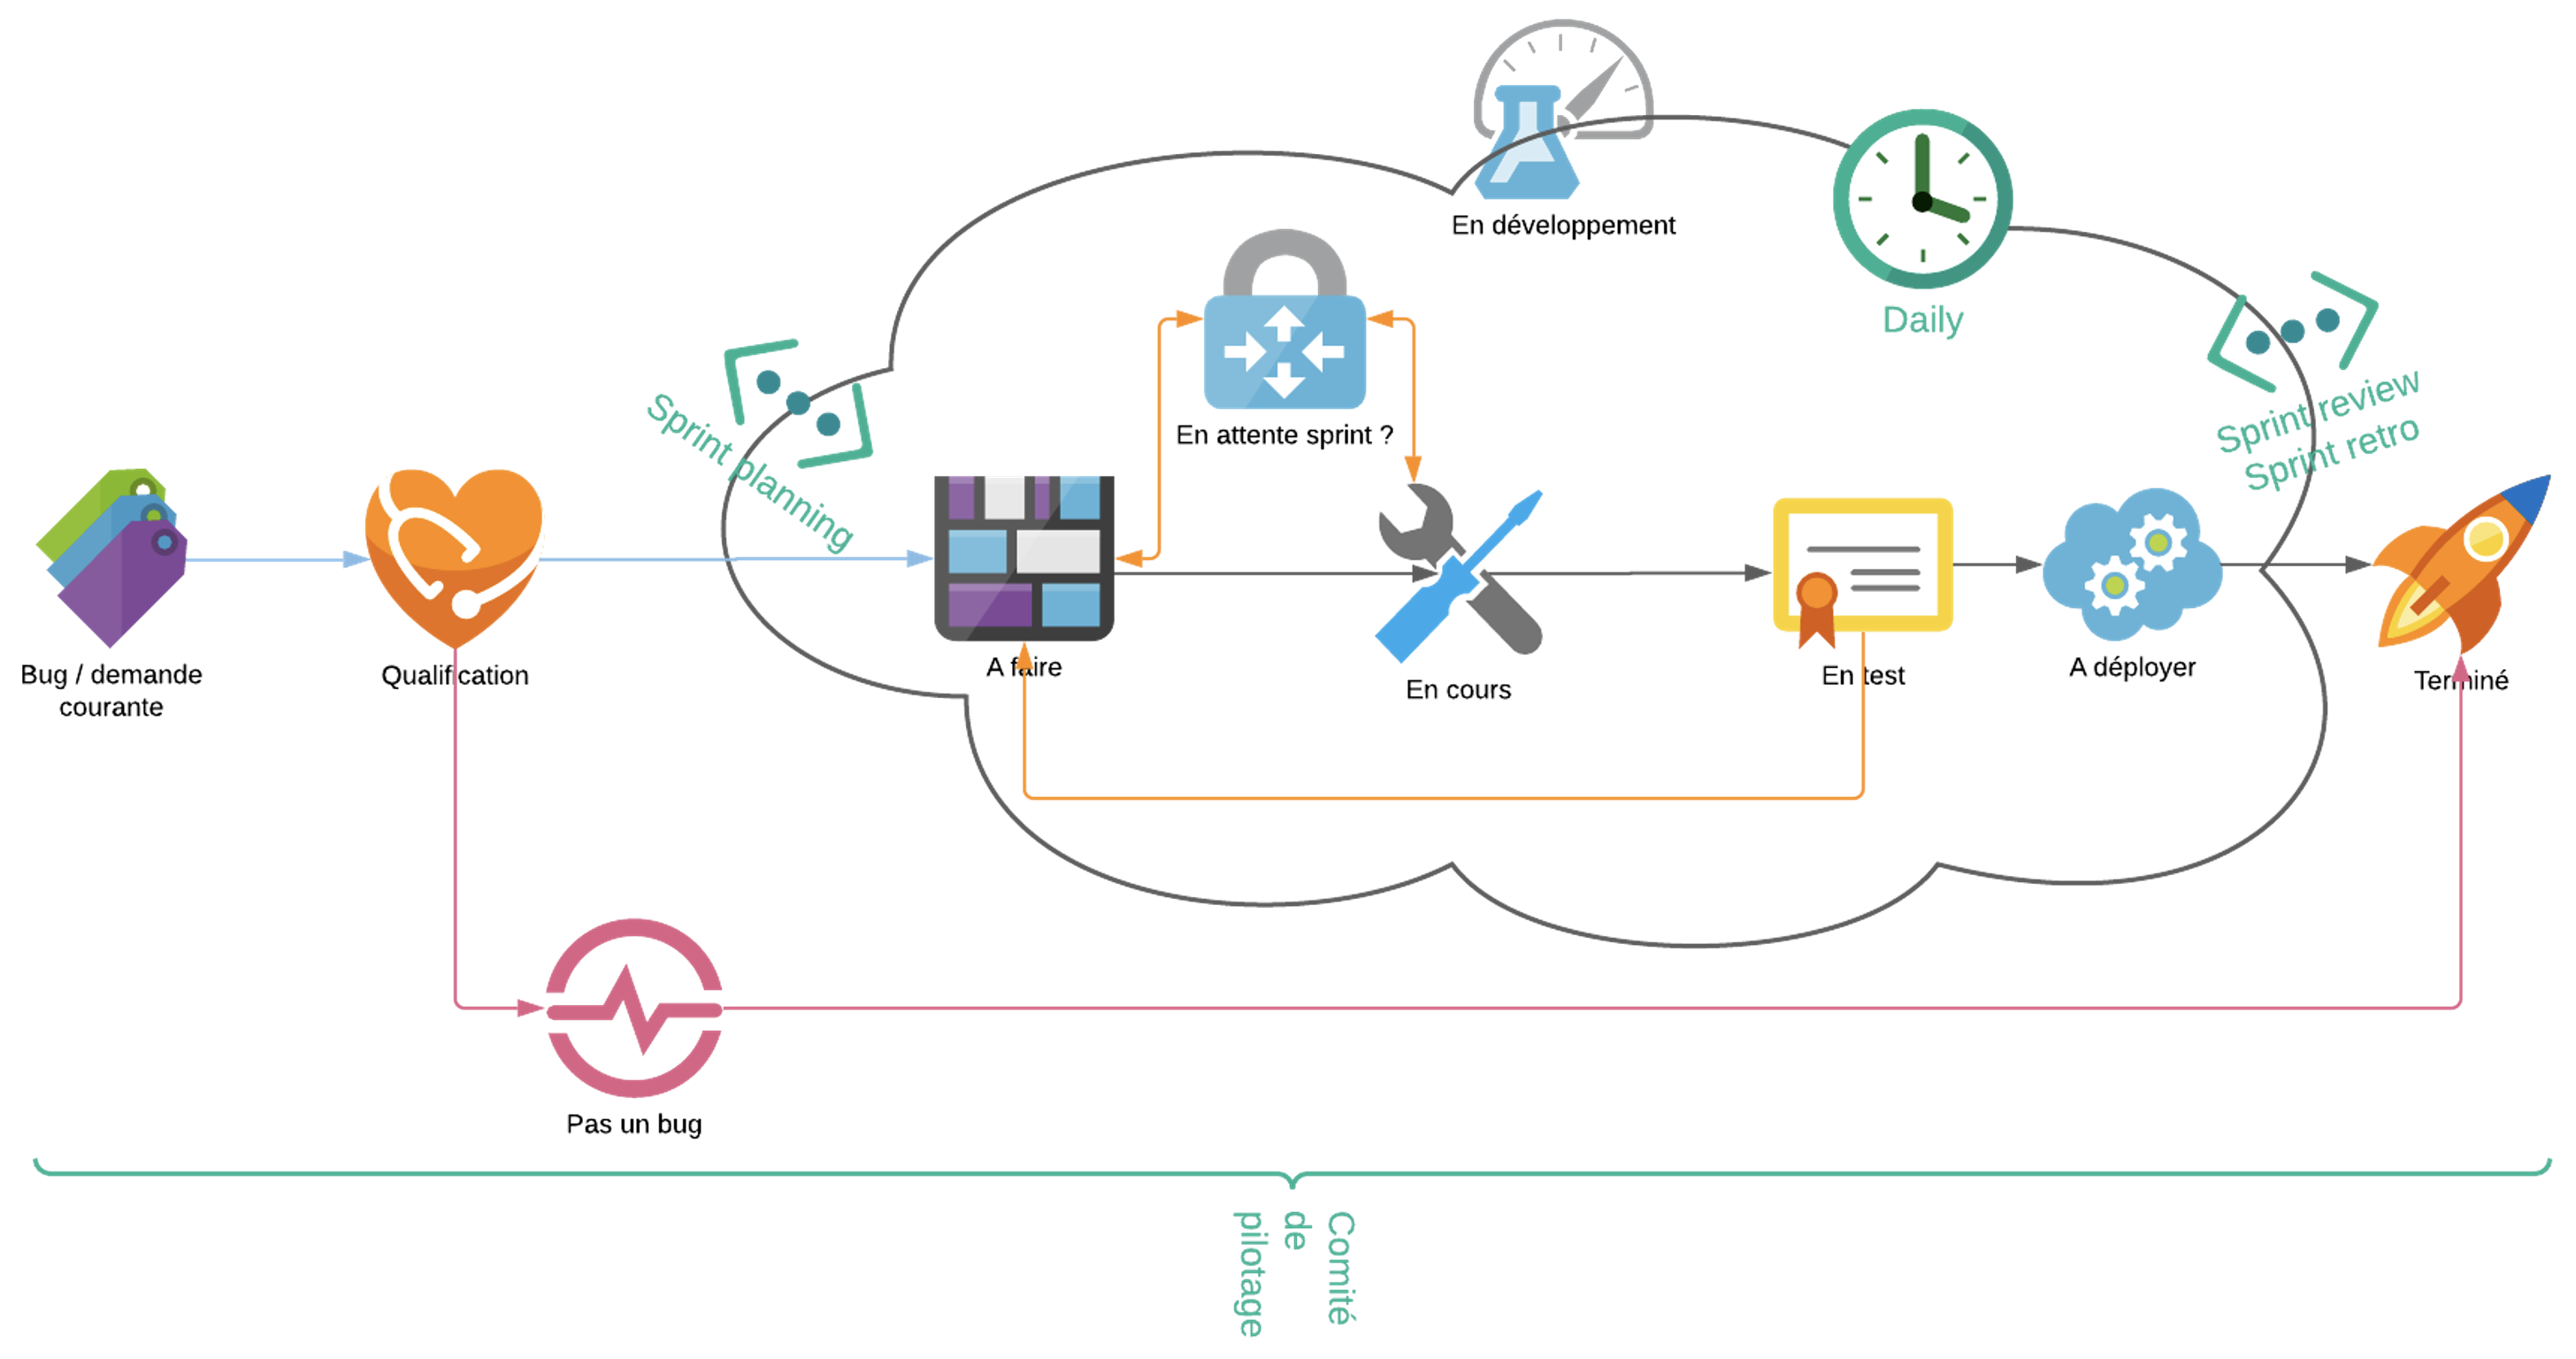
\includegraphics[width=\textwidth]{img/treatment-of-bugs}
    \caption{Diagramme d'activité du traitement des bugs.}
    \label{fig:treatment-of-bugs}
\end{figure}
\section[Jira : L'outil essentiel pour la gestion de projet]{Jira : L'outil essentiel pour la gestion quotidienne de projet}\label{sec:jira}

Au sein de l'entreprise, les équipes SCRUM se servent de Jira afin de consigner et de suivre tous les aspects de leur travail.

Jira est un outil essentiel pour les équipes SCRUM car il facilite la gestion complète du processus de développement agile. Il permet aux équipes de collaborer de manière efficace et de suivre chaque étape du cycle de vie du projet. Avec Jira, les équipes SCRUM peuvent créer, organiser et hiérarchiser leur Carnet de Produit en ajoutant des Histoires Utilisateurs, des tâches, des Épics et des bugs.

L'outil facilite la planification des sprints en permettant aux équipes de sélectionner les éléments du Carnet de Produit à inclure dans chaque itération. Les équipes peuvent estimer la complexité des tâches à l'aide de Story Points et suivre leur progression au fil du temps.

Les fonctionnalités de suivi des tâches et des problèmes dans Jira aident les équipes à gérer leur travail quotidien. Chaque membre de l'équipe peut mettre à jour l'état de ses tâches, signaler les obstacles et collaborer de manière transparente avec les autres membres de l'équipe.

Les réunions SCRUM telles que la Mêlée Quotidienne, la Revue de Sprint et la Rétrospective de Sprint peuvent être orchestrées efficacement grâce à Jira. L'outil permet de suivre les progrès, de partager les résultats et de documenter les réflexions pour chaque itération.

Les flux de travail (workflows) dans Jira constituent un mécanisme central pour orchestrer et suivre le déroulement des tâches et des projets. Ces flux définissent les étapes spécifiques à suivre pour qu'une tâche ou un problème progresse, de sa création à son achèvement. Les équipes peuvent personnaliser ces flux pour refléter leurs processus uniques, en définissant les transitions entre les étapes et en assignant des responsabilités à différents membres de l'équipe. Les flux de travail de Jira contribuent à maintenir la transparence, à améliorer l'efficacité et à garantir que toutes les parties prenantes restent informées de l'avancement du travail. Grâce à cette fonctionnalité, les équipes peuvent gérer avec agilité et précision les tâches, tout en favorisant une collaboration fluide et une visibilité accrue sur les projets.

Chez SuiviDeFlotte, le diagramme d'activité présenté dans les Annexes, dans la Figure~\ref{fig:lifecycle-of-incoming-ideas} (page~\pageref{fig:lifecycle-of-incoming-ideas}) est la base du flux de travail dans Jira. La partie supérieure gauche du diagramme illustre à nouveau le traitement des idées novatrices par les différents comités. En revanche, la partie supérieure droite présente le traitement des bogues (demandes courantes) qui proviennent de l'équipe de support. Ensuite, le propriétaire du produit sélectionne les tickets pour le prochain sprint à partir de l'ensemble des tickets prêts. Ce diagramme contient les étapes suivantes, qui sont utilisées comme étapes du flux de travail dans Jira : en raffinement, à faire, en cours, en test, à déployer, terminé, abandonné.

Un autre diagramme d'activité montre plus en détail le traitement des bogues (Annexes, Figure~\ref{fig:lifecycle-of-bugs}, page~\pageref{fig:lifecycle-of-bugs}). À partir de ce diagramme, nous pouvons ajouter quelques étapes supplémentaires à la liste des étapes du flux de travail : en attente, en attente support.

Le diagramme de flux de travail qui en résulte et qui est actuellement utilisé est présenté à la Figure~\ref{fig:workflow}.

\begin{figure}[ht]
    \centering
    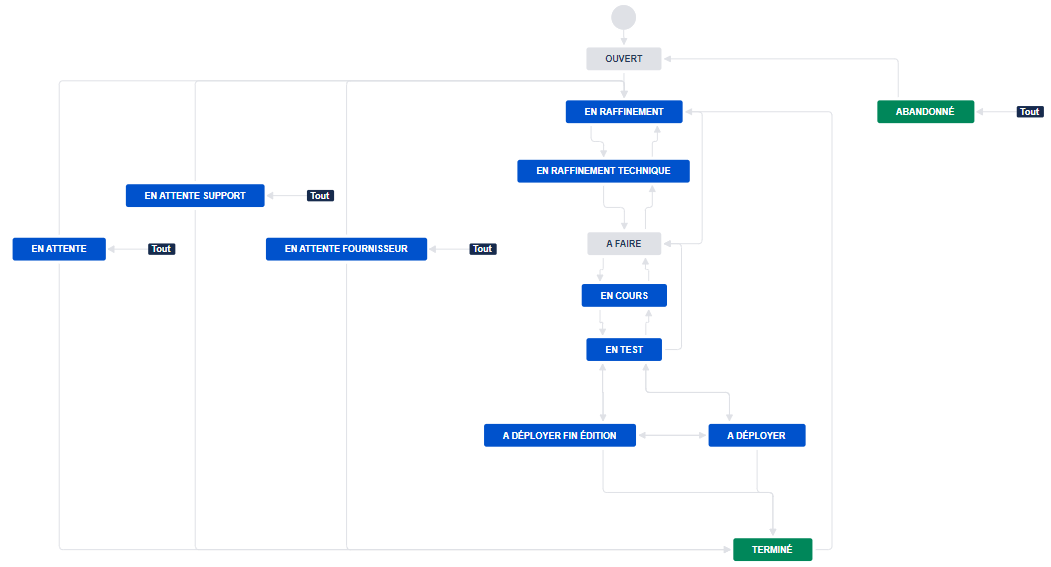
\includegraphics[width=\textwidth]{img/workflow-sdfn}
    \caption{Le flux de travail utilisé dans Jira chez SuiviDeFlotte.}
    \label{fig:workflow}
\end{figure}

Dans les Annexes, la Figure~\ref{fig:product-backlog} (page~\pageref{fig:product-backlog}) et la Figure~\ref{fig:sprint-backlog} (page~\pageref{fig:sprint-backlog}) présentent un exemple de Backlog de produit et de Backlog de sprint sous forme de tableau Kanban, et la Figure~\ref{fig:ticket} (page~\pageref{fig:ticket}) donne un exemple d'un ticket.

\section{Versioning avec Git et GitLab}\label{sec:versioning-git-gitlab}

Dans l'entreprise, les équipes de développement utilisent Git pour la gestion des versions et GitLab pour gérer le processus de développement.

Git est un système de gestion de version décentralisé largement utilisé dans le développement de logiciels. Il permet aux équipes de collaborer efficacement sur des projets en suivant les modifications apportées aux fichiers au fil du temps. Grâce à Git, les développeurs peuvent créer des branches pour travailler sur des fonctionnalités spécifiques ou des corrections de bugs sans perturber le code principal. Les commits, qui représentent des enregistrements de changements, sont la pierre angulaire de Git, permettant de garder une trace claire de l'évolution du code.

GitLab, quant à lui, est une plateforme de gestion de développement logiciel basée sur Git. Elle offre un environnement complet pour le cycle de vie du développement, de la planification à la surveillance. GitLab permet aux équipes de suivre les problèmes, de planifier les sprints, de gérer les demandes d'extraction et de créer des pipelines d'intégration continue pour automatiser les tests et le déploiement. En regroupant toutes ces fonctionnalités au même endroit, GitLab facilite la collaboration entre les membres de l'équipe et permet une gestion transparente et efficace des projets de développement.

Parmi ces nombreuses fonctionnalités, les équipes de DevOps et de développement n'utilisent cependant pas les fonctionnalités de gestion de projet et d'intégration continue/de livraison continue de GitLab, puisqu'elles utilisent Jira (comme nous l'avons vu dans la section précédente) et TeamCity (comme nous le verrons dans la section suivante) à ces fins. GitLab est donc principalement utilisé comme un hébergeur de dépôt de code et un outil de révision de code avec des fonctionnalités telles que les demandes de fusion (merge request).

La Figure~\ref{fig:versioning-and-environments} illustre les principes du versioning et les différents environnements utilisés pour héberger les différentes versions du code. Le tableau Y apporte quelques compléments d'information.

\begin{sidewaysfigure}
    \centering
    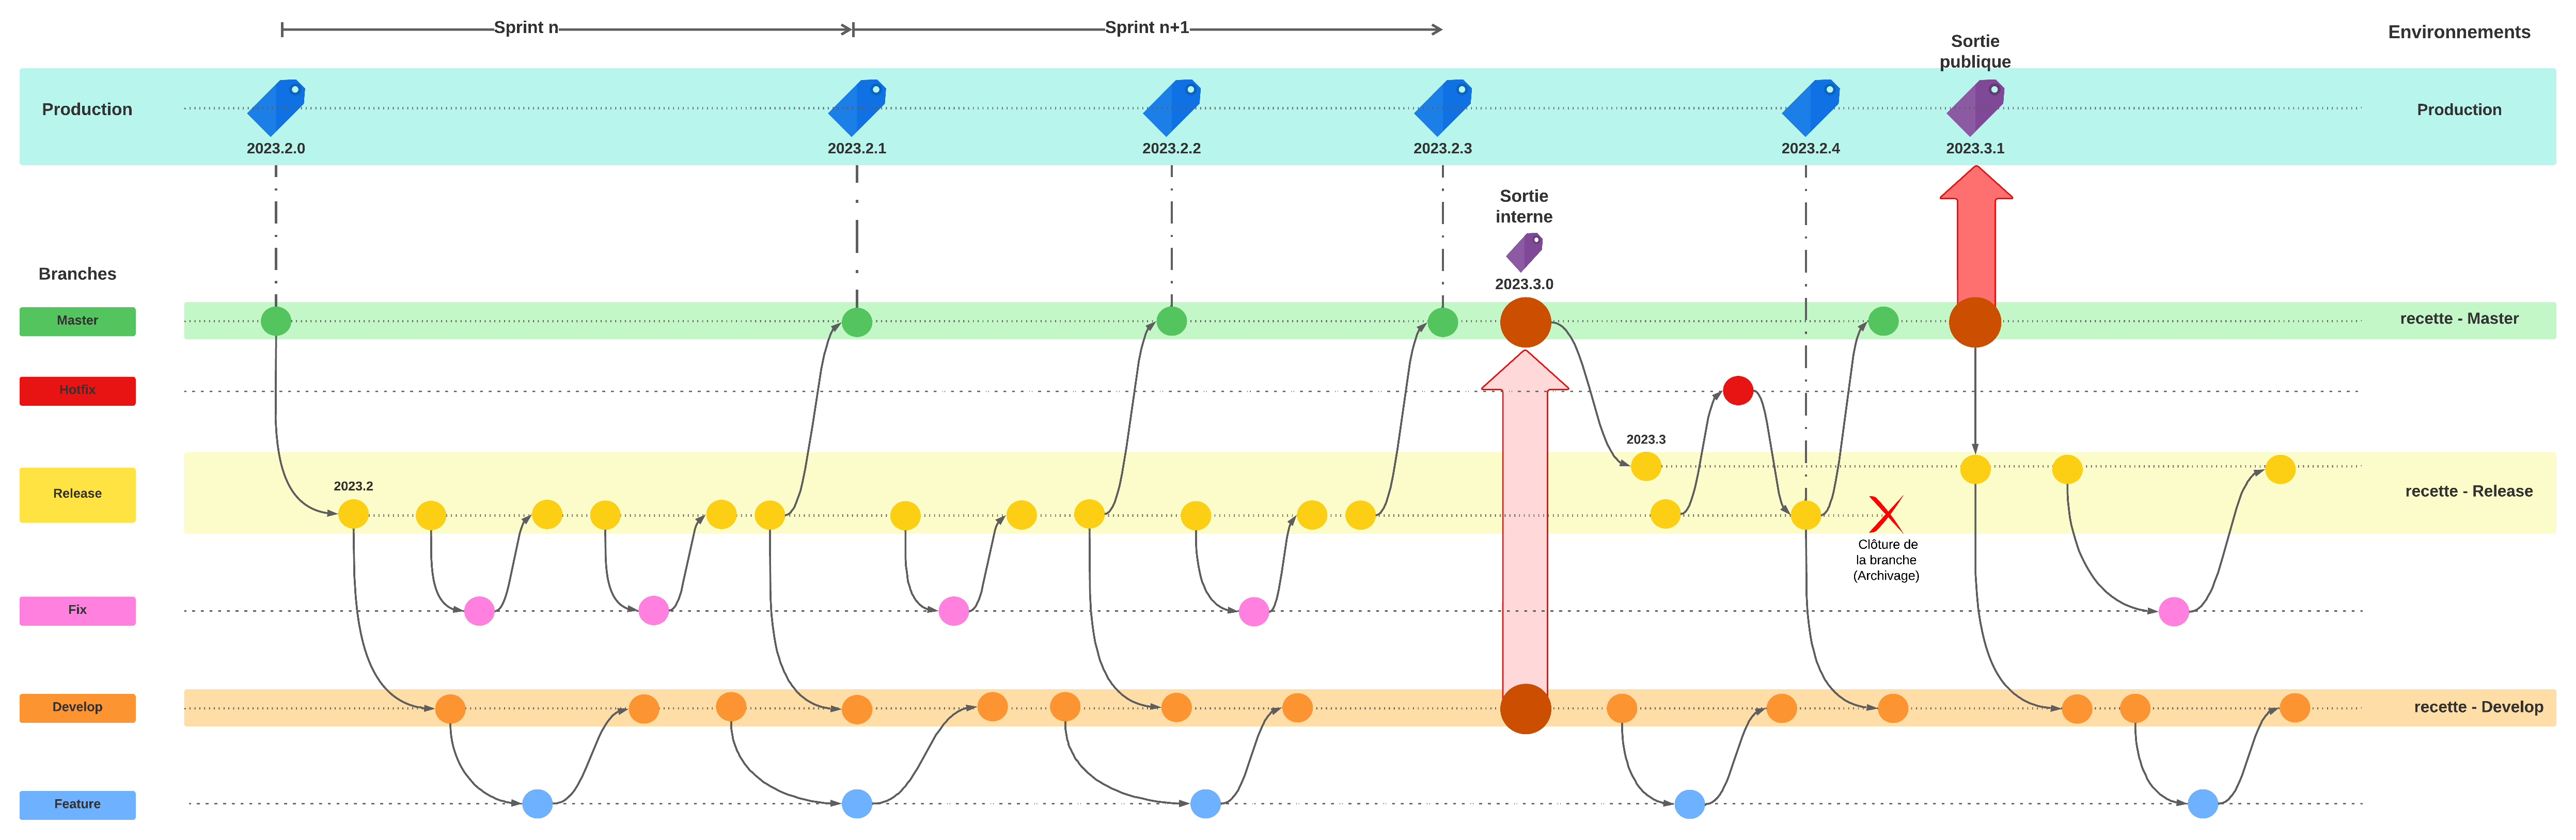
\includegraphics[width=\textwidth]{img/versioning-and-environments}
    \caption{Le schéma du versioning et des environnements.}
    \label{fig:versioning-and-environments}
\end{sidewaysfigure}

\begin{longtblr}[
    caption={Les caractéristiques des différents environnements.},
    label={tblr:environments}
    ]{
    hlines,vlines,
    rowspec={Q[m,font=\footnotesize\bfseries,gray9]*{5}{Q[m,font=\footnotesize]}}
    }
    Environnement    & {Pour quels                       \\ services} & Branches & {Type de \\ comits} & {Déploiement \\ TeamCity} \\
    {Dev pour chaque                                     \\ développeur} & Développeur & {Développeur \\ sandbox} &  & -- \\
    recette-develop  & {Le PO vérifie                    \\ les fonction-\\nalités}                                & develop             & feat                                                         & Auto                                                                      \\
    recette-releases & {Le PO vérifie                    \\ les corrections}                                    & releases/édition    & fix                                                          & Auto                                                                      \\
    recette-master   & {Autres                           \\ services                    \\ pour test \\ (direction, \\ marketing, \\ commerce \\ \dots)} & master              & {(env juste \\ avant la prod, \\ préproduction)}                     & {Manuel, \\ section master \\ dans TeamCity, \\ demande via \\ ticket MEP \\ à DevOps}     \\
    production       &                & tag & {Commit en \\ production \\ avec tag \\ \{numéro-édtion\}.\\\{numéro-increment\}} & {Manuel, \\ section \\ production \\ dans TeamCity, \\ demande via \\ ticket MEP \\ à DevOps}
\end{longtblr}

\section{CI/CD : Intégration Continue et Déploiement Continu}\label{sec:ci-cd}

\section{Cycle de vie d'une nouvelle évolution}\label{sec:cycle-de-vie}